\section{Introduction}\label{sec:srslam:introduction}
%
% With their bodies entirely made of soft deformable materials, continuum soft robots are especially suited for application domains involving safe and robust interaction with humans and environment, and ranging from inspection, to healthcare and agriculture~\citep{majidi2014soft,elfferich2022soft}. To achieve these goals, soft robots must first master the art of controlling and sensing their body shape in space \citep{della2023model}.
\dropcap{A} major challenge with shape perception in soft robots is that sensing strategies must not compromise the intrinsic softness of these systems~\citep{polygerinos2017soft,wang2018toward}. %In the literature they mainly propose resistive, capacitive and magnetic sensors to achieve proprioception \citep{cianchetti2012sensorization,polygerinos2017soft,atalay2017batch,atalay2018highly}.
%
% One way to achieve this goal is to look for . 
To this end, researchers have proposed several entirely deformable sensors over the years, including capacitive~\citep{scimeca2019model} and optical sensors~\citep{li2021scaling}, liquid metal~\citep{wall2017method}. These solutions are quite attractive since they minimally corrupt the physical softness of the robot. However, they usually require complex learning strategies to be used since their behavior is hard to model~\citep{thuruthel2019soft,truby2020distributed}.
%
% wall an brock sousace finger
% moritz otpmized sensing
% 
An alternative is to relax the constraint of complete deformability and allow from small rigid components. This strategy enables rethinking the use of existing sensing technologies in this radically new context. Examples are hall sensors~\citep{guo2019continuum}, IMUs~\citep{hughes2020sensing}, and microphones~\citep{zoller2018acoustic}. %wall and brock
%
The information gathered from inward-facing cameras looking at features in soft chambers' inner walls has proven sufficient to estimate the configuration~\citep{she2020exoskeleton,werner2020vision}, and characterize contacts with the environment \citep{ward2018tactip,lin2020curvature}. However, all these strategies need machine learning to transform the image information in the desired physical quantity.
%
%Classical image filters for feature extraction are combined with \gls{SVR} to estimate a tip position from the camera images. % Their approach performs similarly to a performance baseline made with an off-the-shelf distance sensor used to measure the linear extension.
%
% Another research by \citet{wongwilai2014slam} proposes a framework that combines all grasping tasks (object model acquisition, grasping point calculation and navigation of the robotic arm) with a RGB-D \gls{SLAM}.
%
% In contrast, fewer papers explore the use of camera images for proprioception. \citet{weber2012multi} use an array of micro-cameras which face the environment to estimate the configuration of a single segment robot. The algorithm employs a configuration estimation refinement followed by a full \gls{BA}. 
%
% \citet{cheng2020approximate} present a kinematic equivalent model for a planar continuum robot. They build an Approximate \gls{PCC} model, using classical rigid linkages (2L-5R). They also propose a configuration estimation of the planar continuum robot using a monocular camera as an application to their model.
%
%\textbf{\citep{wang2018robot}} they combine SLAM and manipulation for a humanoid robot (Atlas).
%
%\textbf{\citep{klingensmith2016articulated}} they use RGB-D SLAM for estimating joint angles of an articulated manipulator. 
%
%\textbf{\citep{wongwilai2014slam}} they use SLAM for grasping (depth camera). they combine the process of data acquisition, navigation and grasp point calculation together.
%
Alternatively, cameras mounted outwards on the robot's tip and have been used to execute visual servoing~\citep{homberg2019robust}.
% more citations: wang2013visual
%
To the best of the Authors' knowledge, the only two works dealing with continuum (non-soft) robots are \citep{weber2012multi} and \citep{cheng2020approximate}.
% 
The first uses \gls{BA} to integrate the output of multiple cameras embedded in a single segment. The second uses hand-tuned features to estimate the robot configuration within a novel kinematic model. Thus, no general strategy to estimate the whole state of a soft segment from a single monocular camera exists in the literature.
%
\gls{SLAM} is one of the most effective and largely used strategies for vision-based localization for mobile robots and autonomous vehicles~\citep{fuentes2015visual,mur2017orb}. %SLAM has been used been widely used in autonomous vehicles \citep{x} and rigid robots~\citep{klingensmith2016articulated}.
%
In this chapter, we investigate using monocular \gls{SLAM} to estimate the location of selected points across the soft robot. We then propose a mechanism for simultaneously refining the estimation and reconstructing the complete shape of the robot. We do that by retracting the output of the \gls{SLAM} to the manifold of camera configurations admitted by the kinematic model of the soft robot. We formulate this action as a nonlinear optimization problem. Fig.~\ref{fig:srslam:method_overview} summarizes the proposed architecture. We test the strategy with simulations and experiments, achieving mean relative translational errors between \SI{0.4}{\percent} and \SI{9}{\percent} in the former, and from \SI{5}{\percent} to \SI{9}{\percent} in the latter.

\begin{figure*}[ht]
     \centering
     \subfigure[Overview]{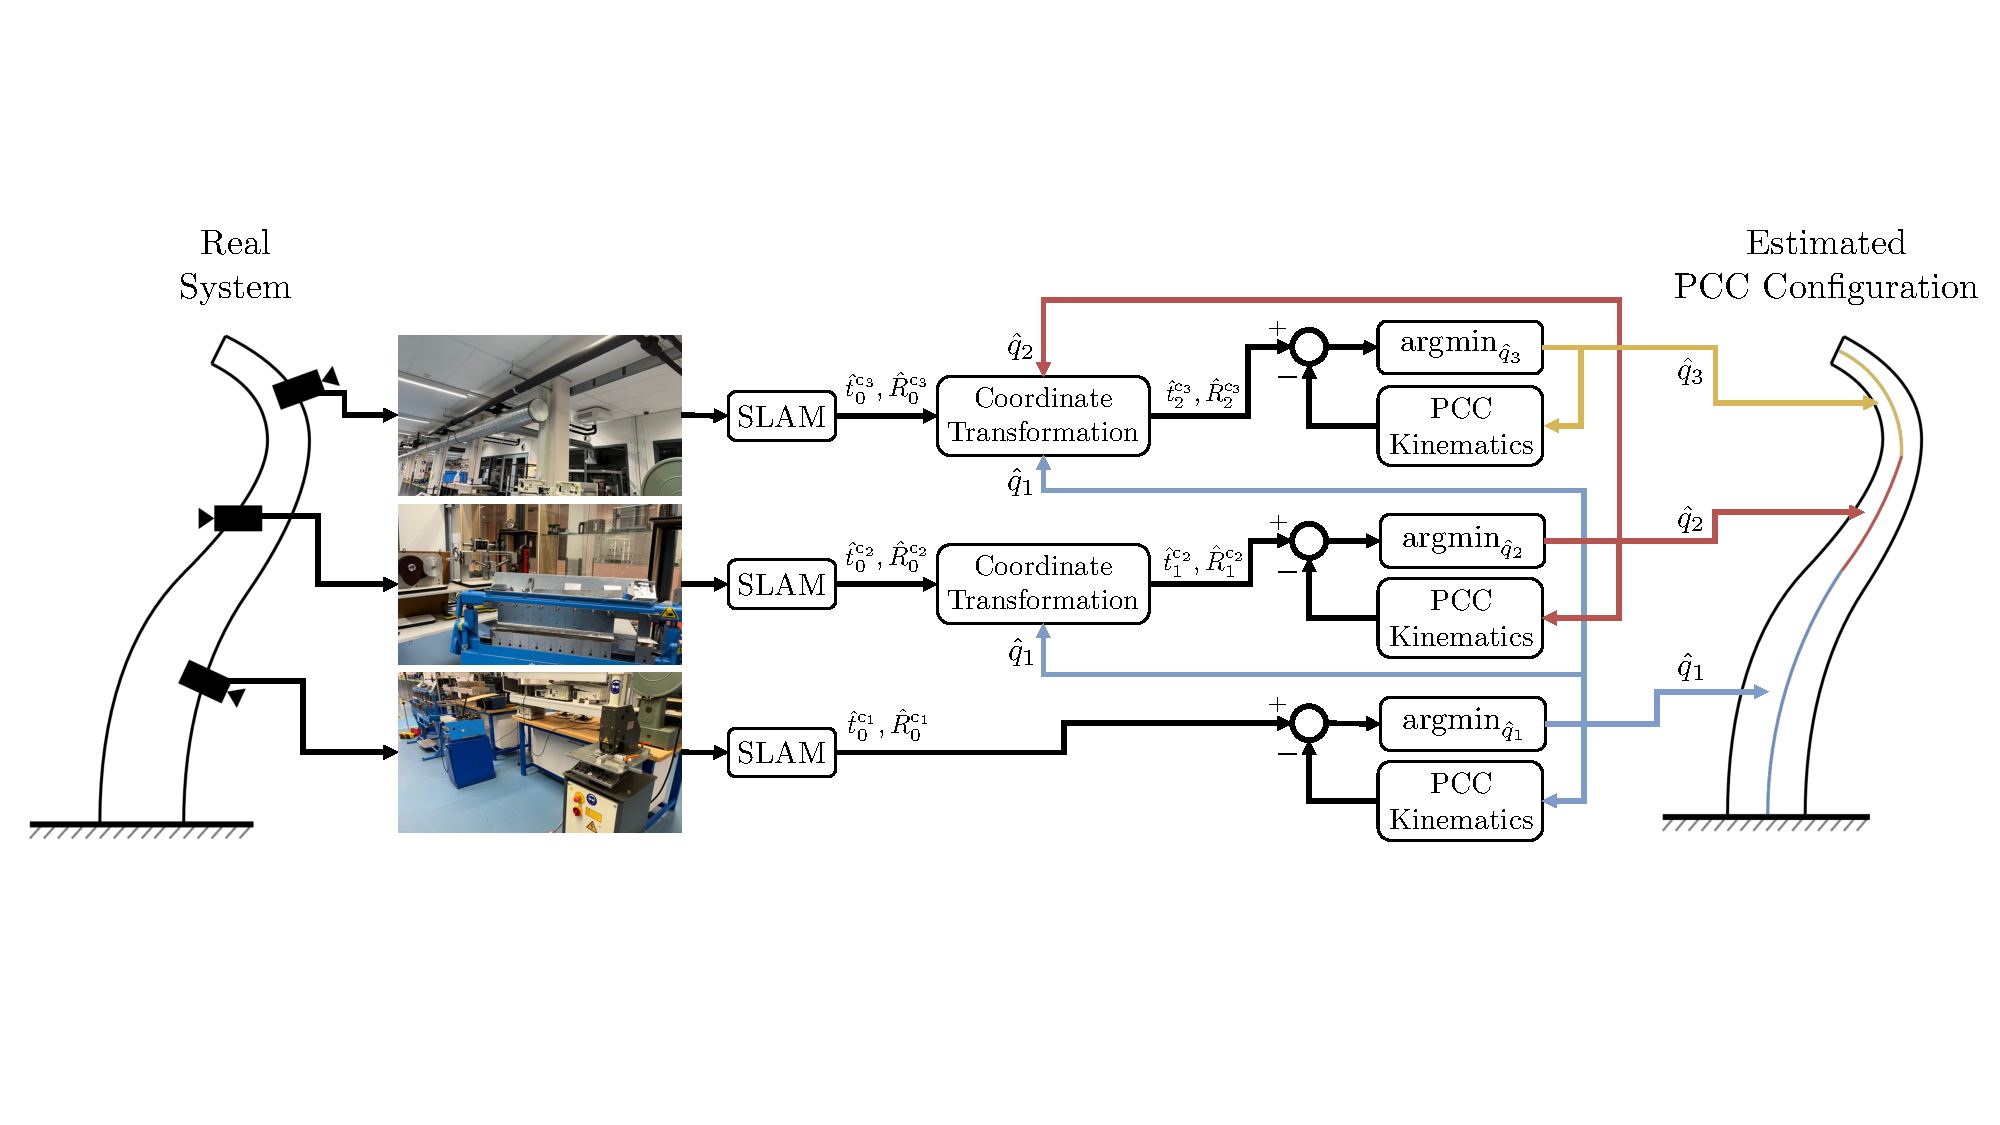
\includegraphics[width=0.69\columnwidth]{srslam/figures/graphic_method_overview_v5_cropped.pdf} \label{fig:srslam:method_overview}}
     \subfigure[Kinematics]{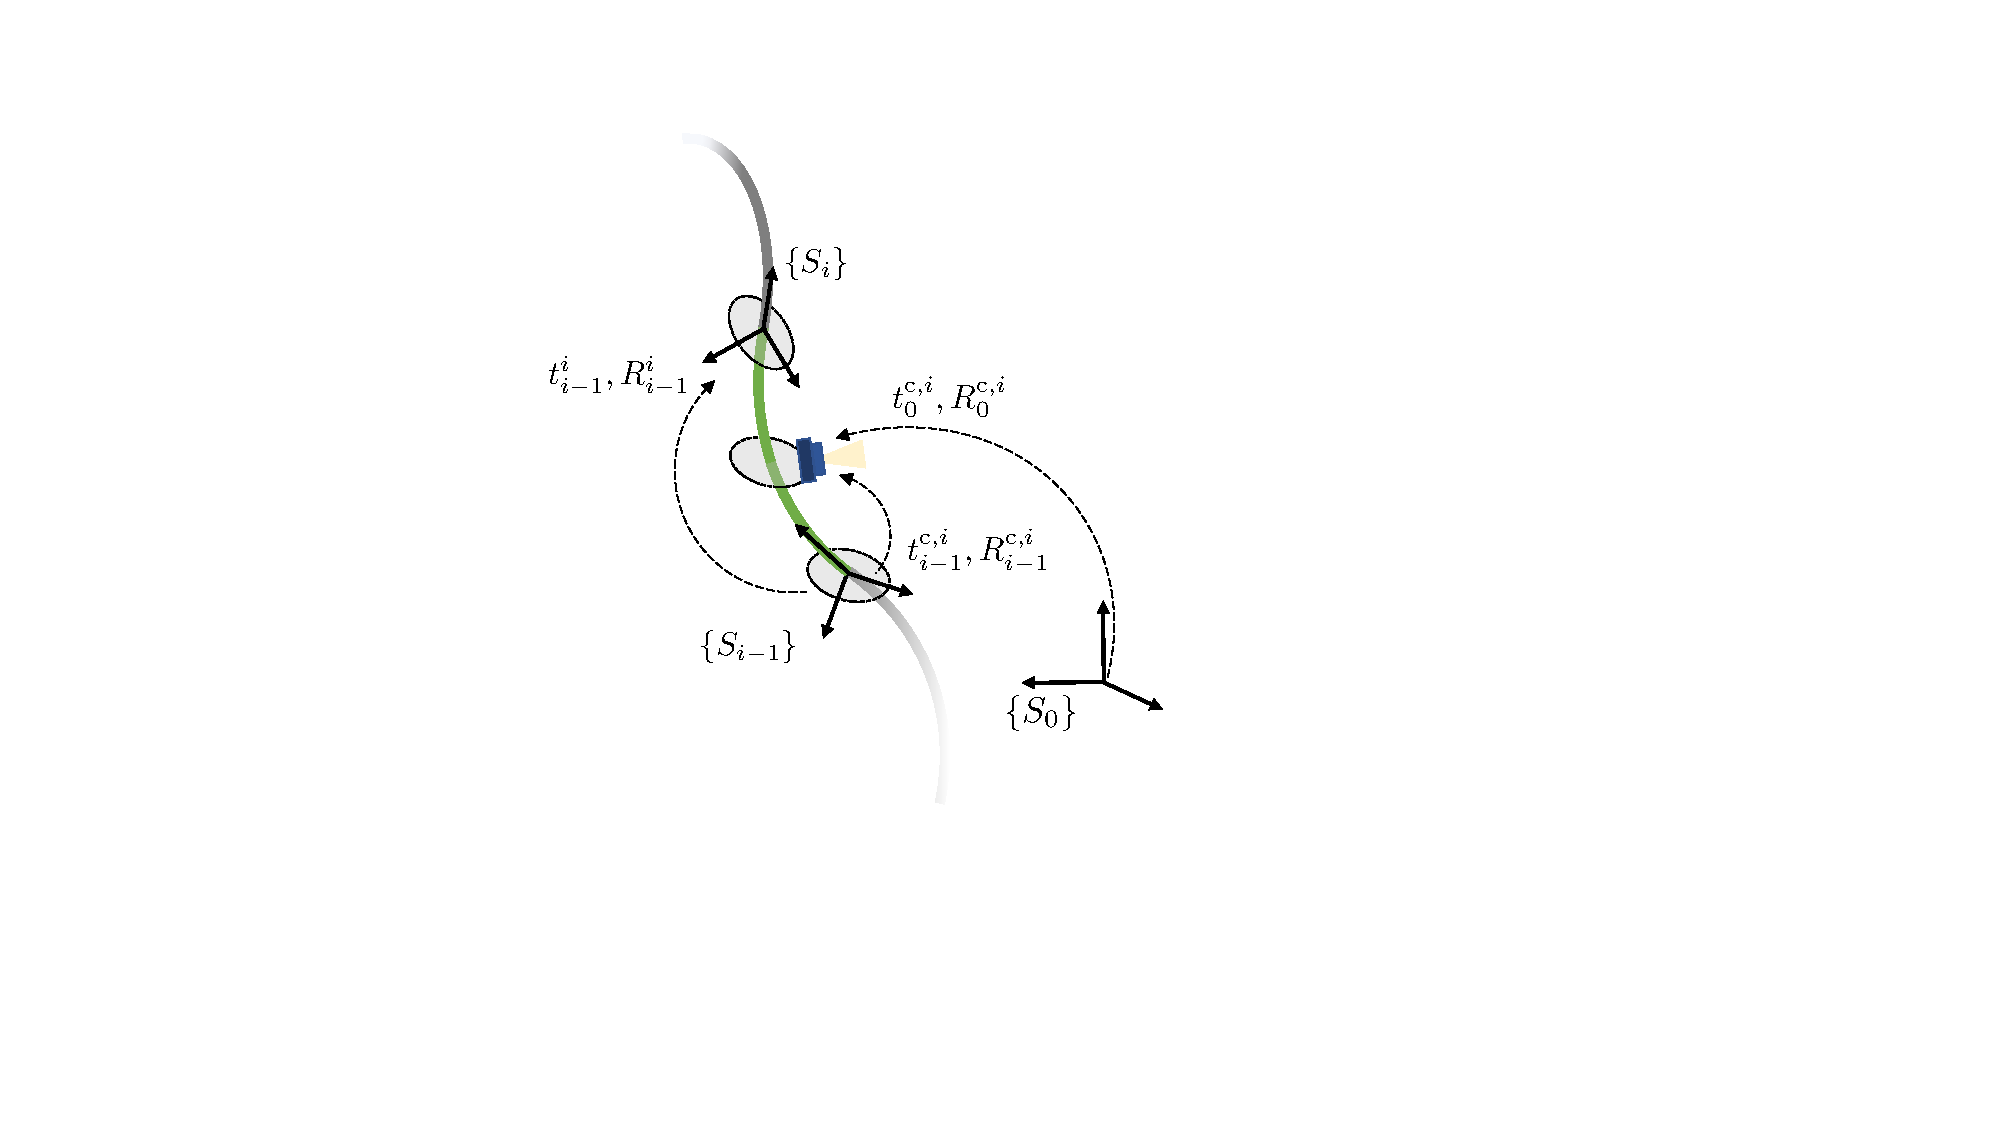
\includegraphics[width=0.24\columnwidth, trim = {0 0 0 0}, clip]{srslam/figures/kinematics_v2.pdf}\label{fig:srslam:kinematic_parameters} \label{fig:srslam:kinematics}}
     \caption{ Panel (a) shows a pictorial representation of the proposed perception strategy. Cameras are attached to a soft continuum robot. We propose to use ORB-SLAM~\citep{mur2017orb} to gather a pose estimate for each camera. The results are iteratively combined to extract local transformation, and refined by projecting the resulting postures onto the manifold of configurations attainable with the \gls{PCC} kinematics. The result is an estimation of the full shape within the selected kinematic description $\hat{q}$. Panel (b) reports the main quantities of the kinematic model of one segment. }
\end{figure*}